\section{RequestHandler Class Reference}
\label{classRequestHandler}\index{RequestHandler@{RequestHandler}}
{\tt \#include $<$request\_\-handler.h$>$}

Inheritance diagram for RequestHandler:\nopagebreak
\begin{figure}[H]
\begin{center}
\leavevmode
\includegraphics[height=400pt]{classRequestHandler__inherit__graph}
\end{center}
\end{figure}
Collaboration diagram for RequestHandler:\nopagebreak
\begin{figure}[H]
\begin{center}
\leavevmode
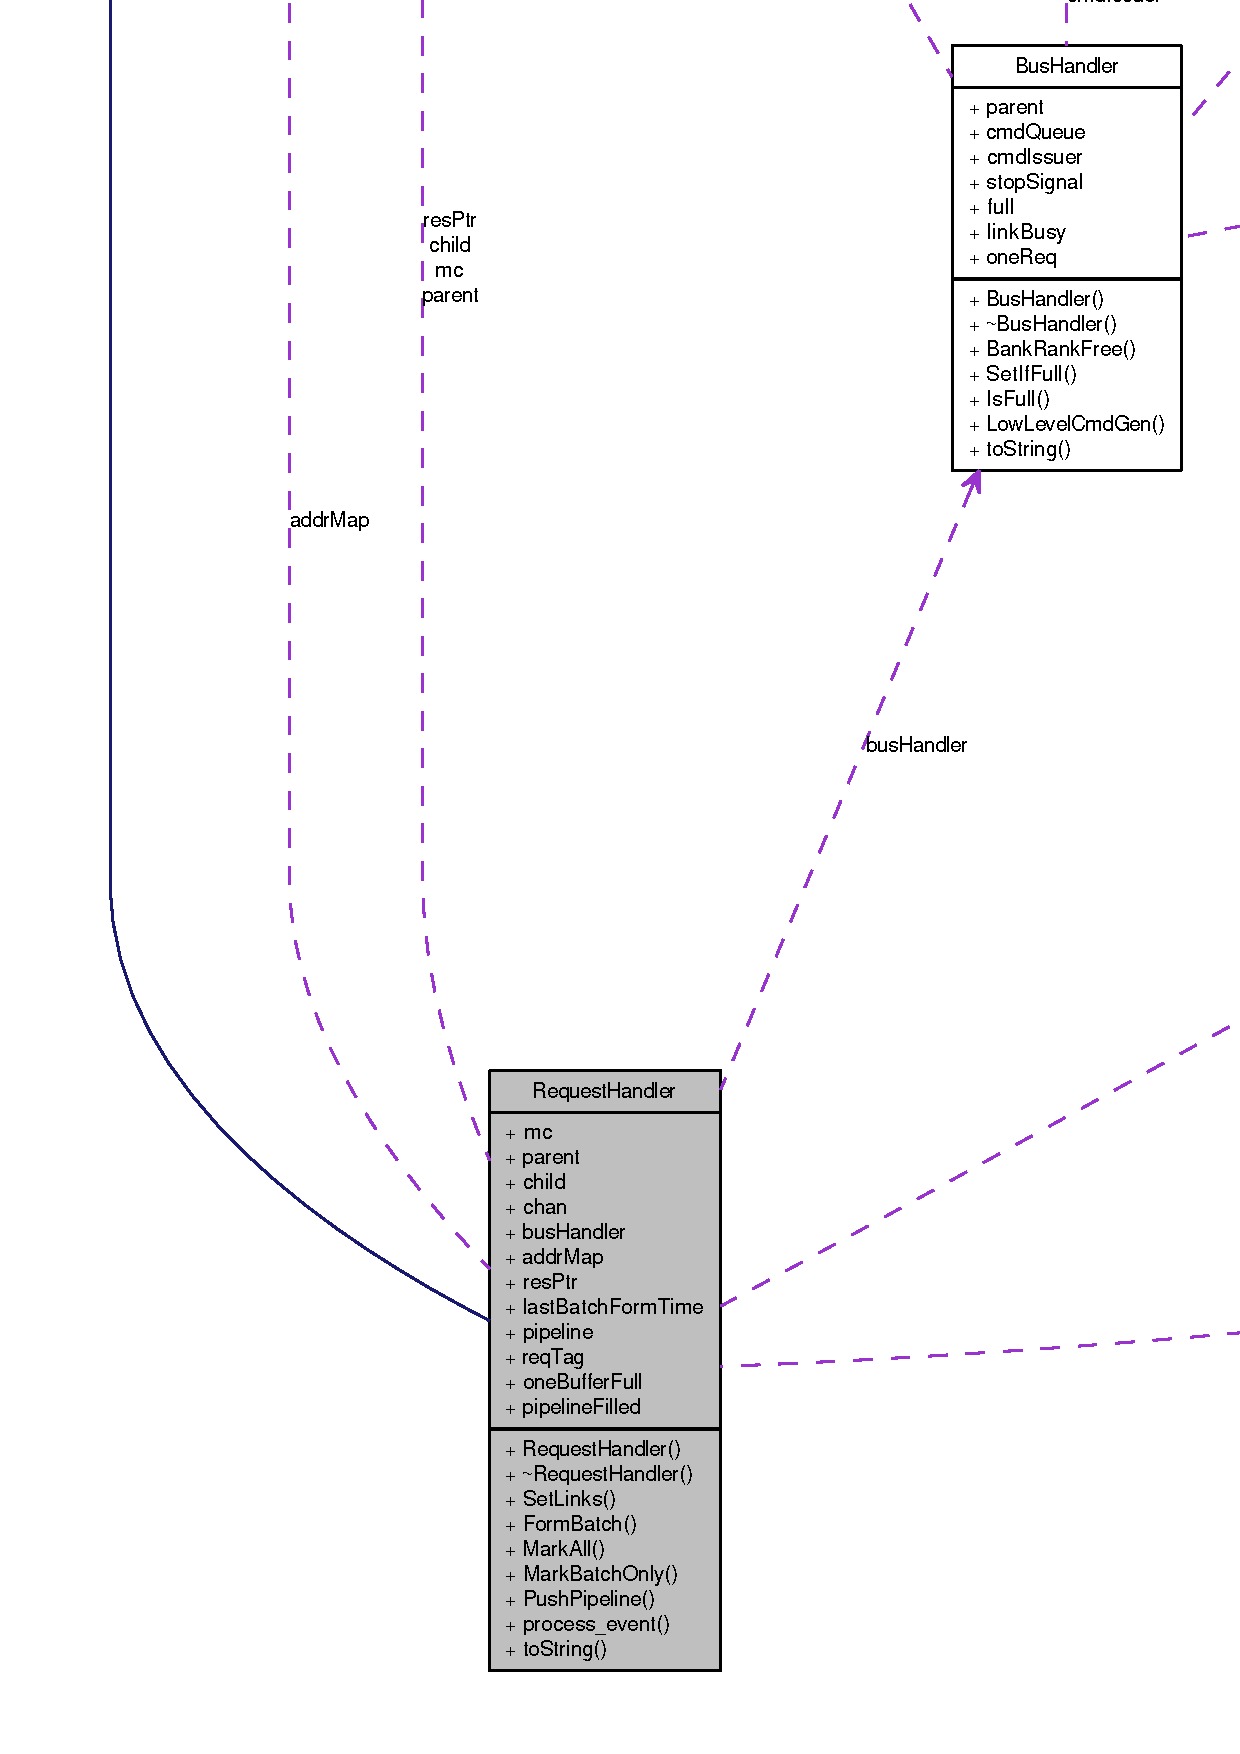
\includegraphics[width=400pt]{classRequestHandler__coll__graph}
\end{center}
\end{figure}
\subsection*{Public Member Functions}
\begin{CompactItemize}
\item 
{\bf RequestHandler} ()
\item 
{\bf $\sim$RequestHandler} ()
\item 
void {\bf SetLinks} ()
\item 
void {\bf FormBatch} ()
\item 
void {\bf MarkAll} ()
\item 
void {\bf MarkBatchOnly} ()
\item 
void {\bf PushPipeline} ({\bf Request} $\ast$req)
\item 
void {\bf process\_\-event} ({\bf IrisEvent} $\ast$e)
\item 
std::string {\bf toString} ()
\end{CompactItemize}
\subsection*{Public Attributes}
\begin{CompactItemize}
\item 
{\bf Component} $\ast$ {\bf mc}
\item 
{\bf Component} $\ast$ {\bf parent}
\item 
{\bf Component} $\ast$ {\bf child}
\item 
{\bf ChannelHandler} {\bf chan} [{\bf NO\_\-OF\_\-CHANNELS}]
\item 
{\bf BusHandler} $\ast$ {\bf busHandler}
\item 
{\bf AddrMap} $\ast$ {\bf addrMap}
\item 
{\bf Component} $\ast$ {\bf resPtr}
\item 
{\bf Time} {\bf lastBatchFormTime}
\item 
{\bf Request} {\bf pipeline}
\item 
int {\bf reqTag}
\item 
bool {\bf oneBufferFull}
\item 
bool {\bf pipelineFilled}
\end{CompactItemize}


\subsection{Detailed Description}


Definition at line 49 of file request\_\-handler.h.

\subsection{Constructor \& Destructor Documentation}
\index{RequestHandler@{RequestHandler}!RequestHandler@{RequestHandler}}
\index{RequestHandler@{RequestHandler}!RequestHandler@{RequestHandler}}
\subsubsection[{RequestHandler}]{\setlength{\rightskip}{0pt plus 5cm}RequestHandler::RequestHandler ()}\label{classRequestHandler_5f47febd4b90dd6fc49b1f8303247c69}




Definition at line 36 of file request\_\-handler.cc.

References addrMap, busHandler, chan, ChannelHandler::chanId, lastBatchFormTime, NO\_\-OF\_\-BANKS, NO\_\-OF\_\-BUFFERS, NO\_\-OF\_\-CHANNELS, NO\_\-OF\_\-RANKS, oneBufferFull, BusHandler::parent, AddrMap::parent, pipelineFilled, ChannelHandler::rank, and reqTag.\index{RequestHandler@{RequestHandler}!$\sim$RequestHandler@{$\sim$RequestHandler}}
\index{$\sim$RequestHandler@{$\sim$RequestHandler}!RequestHandler@{RequestHandler}}
\subsubsection[{$\sim$RequestHandler}]{\setlength{\rightskip}{0pt plus 5cm}RequestHandler::$\sim$RequestHandler ()}\label{classRequestHandler_33488d8c2fa1f2c15193c9918960171a}




Definition at line 71 of file request\_\-handler.cc.

References addrMap, and busHandler.

\subsection{Member Function Documentation}
\index{RequestHandler@{RequestHandler}!FormBatch@{FormBatch}}
\index{FormBatch@{FormBatch}!RequestHandler@{RequestHandler}}
\subsubsection[{FormBatch}]{\setlength{\rightskip}{0pt plus 5cm}void RequestHandler::FormBatch ()}\label{classRequestHandler_29361a7a3ef7c32cc94cb954980229a0}




Definition at line 198 of file request\_\-handler.cc.

References BATCH\_\-FORM\_\-TIME, lastBatchFormTime, and MarkBatchOnly().

Referenced by process\_\-event().

Here is the caller graph for this function:\nopagebreak
\begin{figure}[H]
\begin{center}
\leavevmode
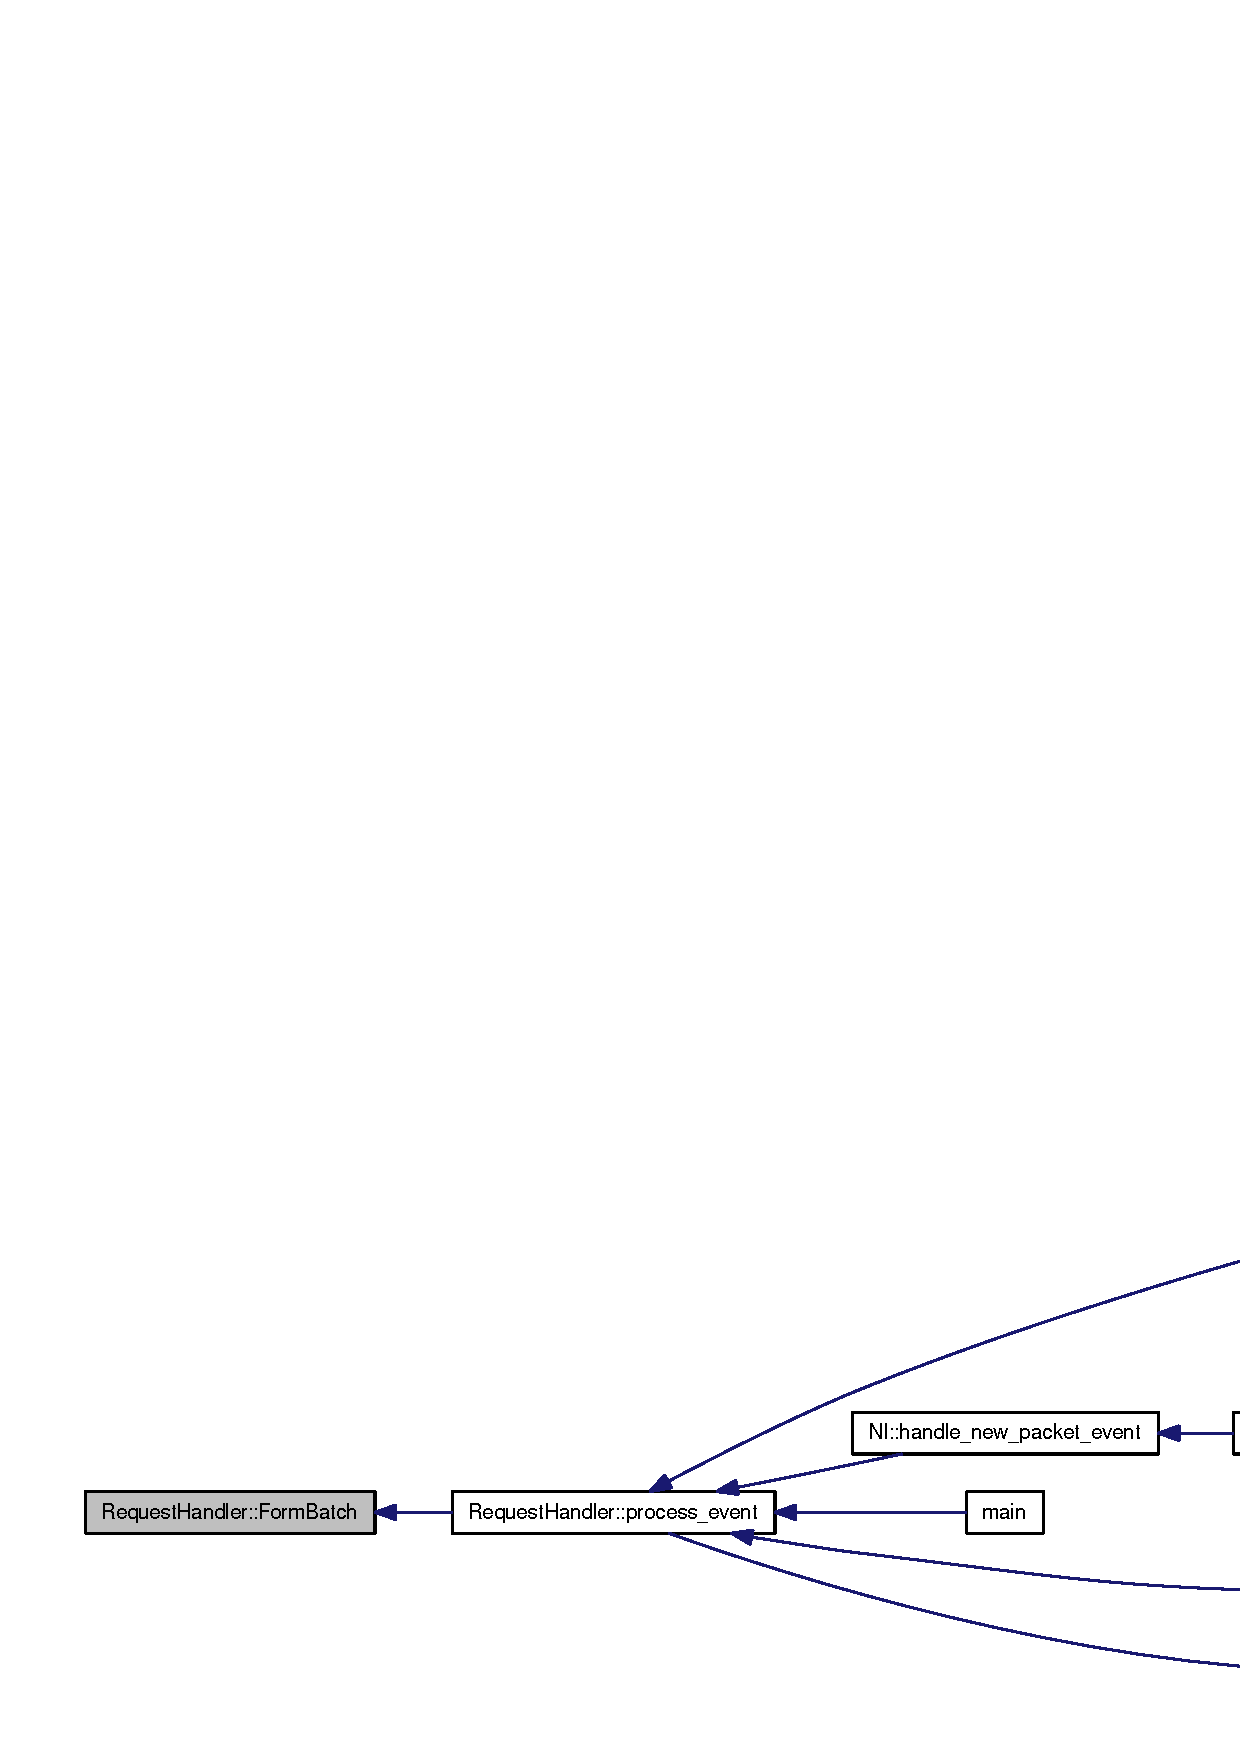
\includegraphics[width=420pt]{classRequestHandler_29361a7a3ef7c32cc94cb954980229a0_icgraph}
\end{center}
\end{figure}
\index{RequestHandler@{RequestHandler}!MarkAll@{MarkAll}}
\index{MarkAll@{MarkAll}!RequestHandler@{RequestHandler}}
\subsubsection[{MarkAll}]{\setlength{\rightskip}{0pt plus 5cm}void RequestHandler::MarkAll ()}\label{classRequestHandler_ebdbb49c40cb699c85f1babb4c88b593}




Definition at line 209 of file request\_\-handler.cc.

References chan, NO\_\-OF\_\-BUFFERS, NO\_\-OF\_\-CHANNELS, NO\_\-OF\_\-RANKS, and ChannelHandler::rank.\index{RequestHandler@{RequestHandler}!MarkBatchOnly@{MarkBatchOnly}}
\index{MarkBatchOnly@{MarkBatchOnly}!RequestHandler@{RequestHandler}}
\subsubsection[{MarkBatchOnly}]{\setlength{\rightskip}{0pt plus 5cm}void RequestHandler::MarkBatchOnly ()}\label{classRequestHandler_7333638ede01b551db94364367a40599}




Definition at line 218 of file request\_\-handler.cc.

References chan, MAX\_\-BATCH\_\-SIZE, NO\_\-OF\_\-BUFFERS, NO\_\-OF\_\-CHANNELS, NO\_\-OF\_\-RANKS, NO\_\-OF\_\-THREADS, and ChannelHandler::rank.

Referenced by FormBatch().

Here is the caller graph for this function:\nopagebreak
\begin{figure}[H]
\begin{center}
\leavevmode
\includegraphics[width=420pt]{classRequestHandler_7333638ede01b551db94364367a40599_icgraph}
\end{center}
\end{figure}
\index{RequestHandler@{RequestHandler}!process\_\-event@{process\_\-event}}
\index{process\_\-event@{process\_\-event}!RequestHandler@{RequestHandler}}
\subsubsection[{process\_\-event}]{\setlength{\rightskip}{0pt plus 5cm}void RequestHandler::process\_\-event ({\bf IrisEvent} $\ast$ {\em e})}\label{classRequestHandler_c295b7e01ed866b390c93a559f375b2f}




Definition at line 86 of file request\_\-handler.cc.

References Request::address, addrMap, BATCH\_\-FORM\_\-TIME, busHandler, CONTINUE, IrisEvent::event\_\-data, FormBatch(), BusHandler::full, lastBatchFormTime, NO\_\-OF\_\-CHANNELS, Simulator::Now(), oneBufferFull, pipeline, pipelineFilled, AddrMap::process\_\-event(), PushPipeline(), Simulator::Schedule(), START, START\_\-CMD\_\-QUEUE, STOP\_\-CMD\_\-QUEUE, BusHandler::stopSignal, and IrisEvent::type.

Referenced by NI::handle\_\-new\_\-packet\_\-event(), main(), BankHandler::process\_\-event(), and MC::sim\_\-main().

Here is the caller graph for this function:\nopagebreak
\begin{figure}[H]
\begin{center}
\leavevmode
\includegraphics[width=420pt]{classRequestHandler_c295b7e01ed866b390c93a559f375b2f_icgraph}
\end{center}
\end{figure}
\index{RequestHandler@{RequestHandler}!PushPipeline@{PushPipeline}}
\index{PushPipeline@{PushPipeline}!RequestHandler@{RequestHandler}}
\subsubsection[{PushPipeline}]{\setlength{\rightskip}{0pt plus 5cm}void RequestHandler::PushPipeline ({\bf Request} $\ast$ {\em req})}\label{classRequestHandler_a3cfb7f3392498247527d307e49d4418}




Definition at line 188 of file request\_\-handler.cc.

References pipeline.

Referenced by process\_\-event().

Here is the caller graph for this function:\nopagebreak
\begin{figure}[H]
\begin{center}
\leavevmode
\includegraphics[width=420pt]{classRequestHandler_a3cfb7f3392498247527d307e49d4418_icgraph}
\end{center}
\end{figure}
\index{RequestHandler@{RequestHandler}!SetLinks@{SetLinks}}
\index{SetLinks@{SetLinks}!RequestHandler@{RequestHandler}}
\subsubsection[{SetLinks}]{\setlength{\rightskip}{0pt plus 5cm}void RequestHandler::SetLinks ()}\label{classRequestHandler_9496685187c3ae6632525b7213fe85c6}




Definition at line 77 of file request\_\-handler.cc.

References busHandler, child, CmdIssuer::cmdBus, BusHandler::cmdIssuer, CmdIssuer::dataBus, and NO\_\-OF\_\-CHANNELS.

Referenced by MC::Init().

Here is the caller graph for this function:\nopagebreak
\begin{figure}[H]
\begin{center}
\leavevmode
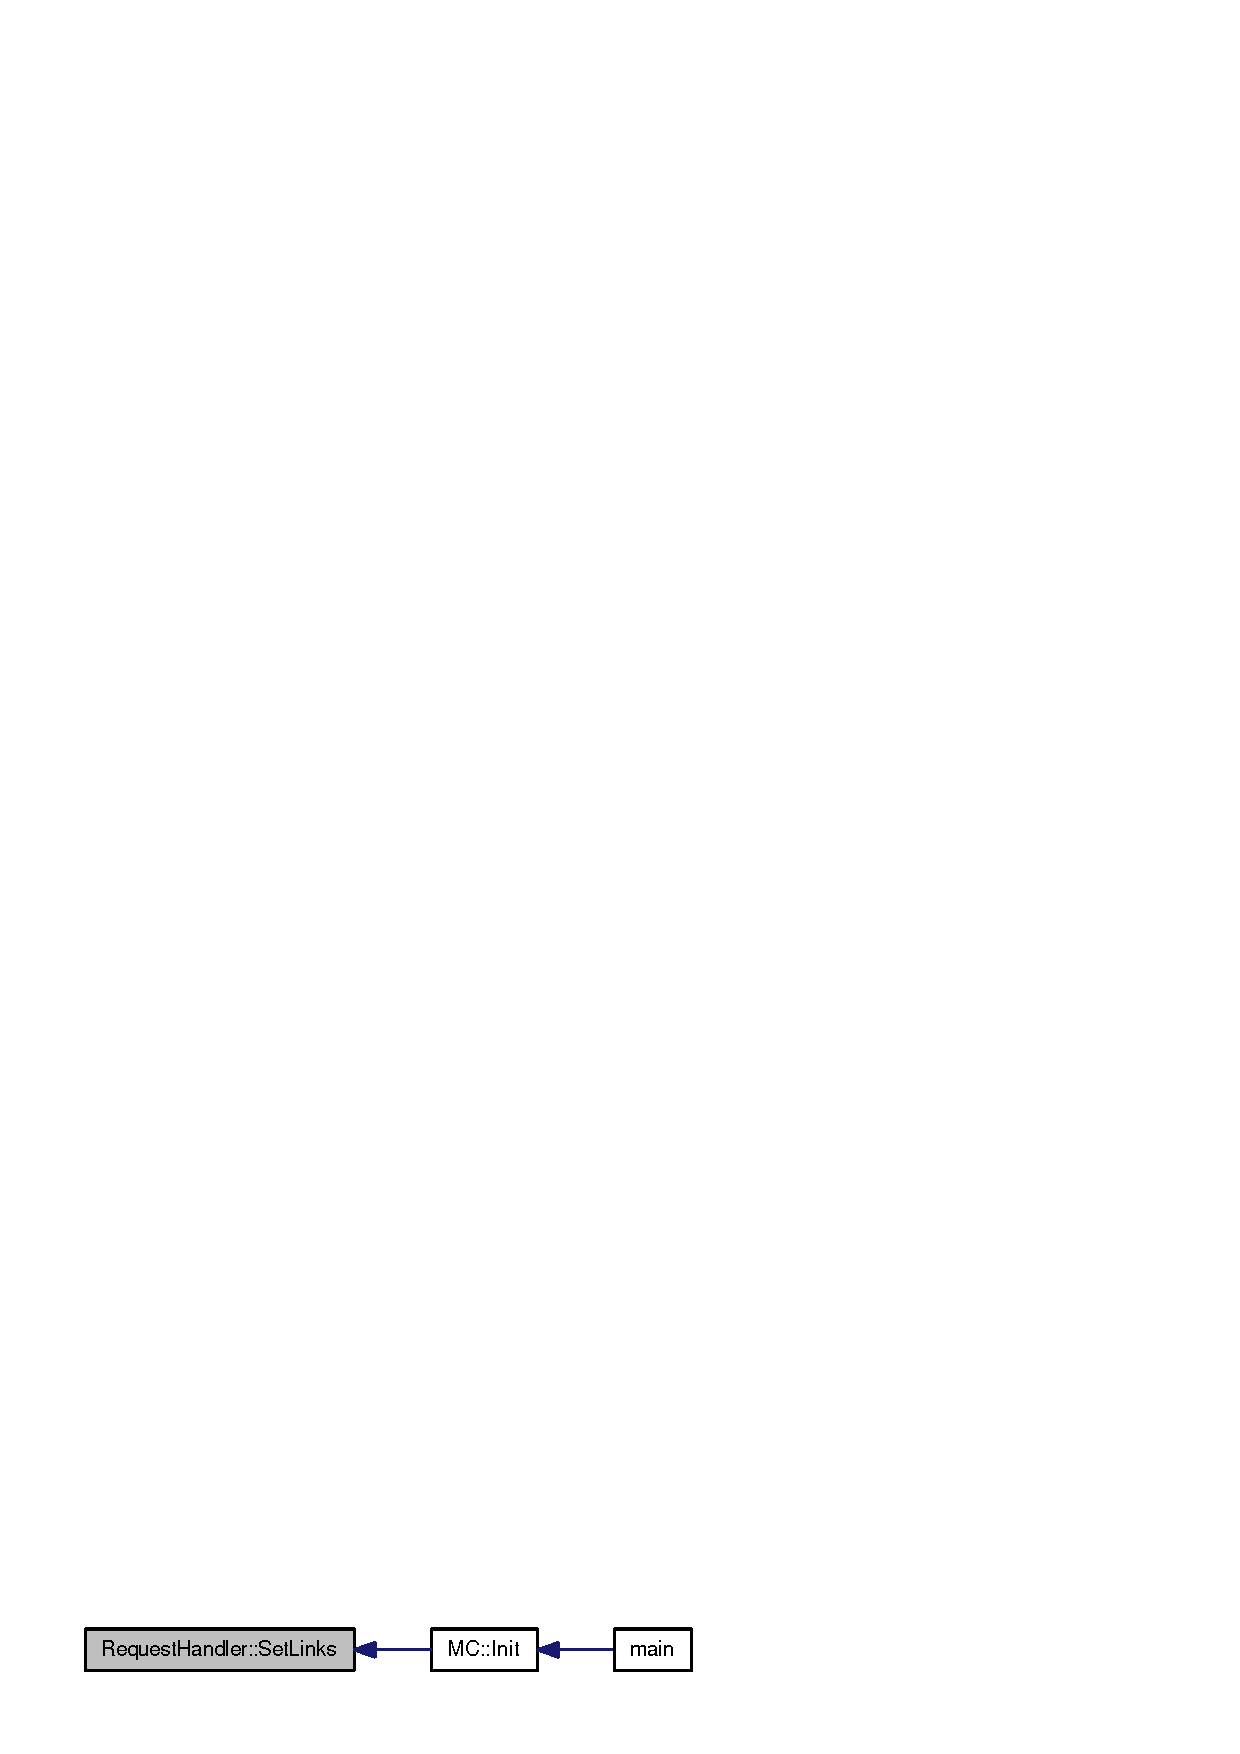
\includegraphics[width=168pt]{classRequestHandler_9496685187c3ae6632525b7213fe85c6_icgraph}
\end{center}
\end{figure}
\index{RequestHandler@{RequestHandler}!toString@{toString}}
\index{toString@{toString}!RequestHandler@{RequestHandler}}
\subsubsection[{toString}]{\setlength{\rightskip}{0pt plus 5cm}std::string RequestHandler::toString ()}\label{classRequestHandler_e4ec28c4cc1247cae927f9fc2a43dad7}




Definition at line 193 of file request\_\-handler.cc.

\subsection{Member Data Documentation}
\index{RequestHandler@{RequestHandler}!addrMap@{addrMap}}
\index{addrMap@{addrMap}!RequestHandler@{RequestHandler}}
\subsubsection[{addrMap}]{\setlength{\rightskip}{0pt plus 5cm}{\bf AddrMap}$\ast$ {\bf RequestHandler::addrMap}}\label{classRequestHandler_7a16df768f3c6ad8aba05a35e1ae9a46}




Definition at line 59 of file request\_\-handler.h.

Referenced by process\_\-event(), RequestHandler(), and $\sim$RequestHandler().\index{RequestHandler@{RequestHandler}!busHandler@{busHandler}}
\index{busHandler@{busHandler}!RequestHandler@{RequestHandler}}
\subsubsection[{busHandler}]{\setlength{\rightskip}{0pt plus 5cm}{\bf BusHandler}$\ast$ {\bf RequestHandler::busHandler}}\label{classRequestHandler_8ede46daf657b02d2eb5fc85fc499c0a}




Definition at line 58 of file request\_\-handler.h.

Referenced by process\_\-event(), RefreshMgr::process\_\-event(), RequestHandler(), SetLinks(), and $\sim$RequestHandler().\index{RequestHandler@{RequestHandler}!chan@{chan}}
\index{chan@{chan}!RequestHandler@{RequestHandler}}
\subsubsection[{chan}]{\setlength{\rightskip}{0pt plus 5cm}{\bf ChannelHandler} {\bf RequestHandler::chan}[{\bf NO\_\-OF\_\-CHANNELS}]}\label{classRequestHandler_ce2dff9fc4bc90740663ab1b5c6d1a02}




Definition at line 57 of file request\_\-handler.h.

Referenced by MarkAll(), MarkBatchOnly(), and RequestHandler().\index{RequestHandler@{RequestHandler}!child@{child}}
\index{child@{child}!RequestHandler@{RequestHandler}}
\subsubsection[{child}]{\setlength{\rightskip}{0pt plus 5cm}{\bf Component}$\ast$ {\bf RequestHandler::child}}\label{classRequestHandler_f1ac97204e61fc5e487a0321fb0fcd7a}




Definition at line 56 of file request\_\-handler.h.

Referenced by MC::Init(), and SetLinks().\index{RequestHandler@{RequestHandler}!lastBatchFormTime@{lastBatchFormTime}}
\index{lastBatchFormTime@{lastBatchFormTime}!RequestHandler@{RequestHandler}}
\subsubsection[{lastBatchFormTime}]{\setlength{\rightskip}{0pt plus 5cm}{\bf Time} {\bf RequestHandler::lastBatchFormTime}}\label{classRequestHandler_71b4ced7b007998a6f65f5ee1e09925a}




Definition at line 61 of file request\_\-handler.h.

Referenced by FormBatch(), process\_\-event(), and RequestHandler().\index{RequestHandler@{RequestHandler}!mc@{mc}}
\index{mc@{mc}!RequestHandler@{RequestHandler}}
\subsubsection[{mc}]{\setlength{\rightskip}{0pt plus 5cm}{\bf Component}$\ast$ {\bf RequestHandler::mc}}\label{classRequestHandler_5e03befd33a2704212d01cc030666ce3}




Definition at line 54 of file request\_\-handler.h.

Referenced by MC::Init().\index{RequestHandler@{RequestHandler}!oneBufferFull@{oneBufferFull}}
\index{oneBufferFull@{oneBufferFull}!RequestHandler@{RequestHandler}}
\subsubsection[{oneBufferFull}]{\setlength{\rightskip}{0pt plus 5cm}bool {\bf RequestHandler::oneBufferFull}}\label{classRequestHandler_8d97d715ba10ab051886b1b5a5b56d68}




Definition at line 64 of file request\_\-handler.h.

Referenced by main(), process\_\-event(), RequestHandler(), and MC::sim\_\-main().\index{RequestHandler@{RequestHandler}!parent@{parent}}
\index{parent@{parent}!RequestHandler@{RequestHandler}}
\subsubsection[{parent}]{\setlength{\rightskip}{0pt plus 5cm}{\bf Component}$\ast$ {\bf RequestHandler::parent}}\label{classRequestHandler_d0c3f57518617d211524ebe7d4da51ef}




Definition at line 55 of file request\_\-handler.h.

Referenced by MC::Init().\index{RequestHandler@{RequestHandler}!pipeline@{pipeline}}
\index{pipeline@{pipeline}!RequestHandler@{RequestHandler}}
\subsubsection[{pipeline}]{\setlength{\rightskip}{0pt plus 5cm}{\bf Request} {\bf RequestHandler::pipeline}}\label{classRequestHandler_dc25794d3e70e92d98d0f424a46cd861}




Definition at line 62 of file request\_\-handler.h.

Referenced by process\_\-event(), and PushPipeline().\index{RequestHandler@{RequestHandler}!pipelineFilled@{pipelineFilled}}
\index{pipelineFilled@{pipelineFilled}!RequestHandler@{RequestHandler}}
\subsubsection[{pipelineFilled}]{\setlength{\rightskip}{0pt plus 5cm}bool {\bf RequestHandler::pipelineFilled}}\label{classRequestHandler_50c874e27d09067976a7da4020c651a7}




Definition at line 65 of file request\_\-handler.h.

Referenced by process\_\-event(), and RequestHandler().\index{RequestHandler@{RequestHandler}!reqTag@{reqTag}}
\index{reqTag@{reqTag}!RequestHandler@{RequestHandler}}
\subsubsection[{reqTag}]{\setlength{\rightskip}{0pt plus 5cm}int {\bf RequestHandler::reqTag}}\label{classRequestHandler_165285c7219bb2a76b9a4ba33c230e0d}




Definition at line 63 of file request\_\-handler.h.

Referenced by RequestHandler().\index{RequestHandler@{RequestHandler}!resPtr@{resPtr}}
\index{resPtr@{resPtr}!RequestHandler@{RequestHandler}}
\subsubsection[{resPtr}]{\setlength{\rightskip}{0pt plus 5cm}{\bf Component}$\ast$ {\bf RequestHandler::resPtr}}\label{classRequestHandler_5ea8057f932d231a2263d45be00489ea}




Definition at line 60 of file request\_\-handler.h.

Referenced by MC::Init().

The documentation for this class was generated from the following files:\begin{CompactItemize}
\item 
{\bf request\_\-handler.h}\item 
{\bf request\_\-handler.cc}\end{CompactItemize}
